\section{Training Details}\label{sec:training_outline}
Here we catalogue details regarding all tasks, datasets, models, batch schedules, and other hyper-parameters used in our experiments. In all experiments, we try to copy as many hyper-parameters from the original papers as possible.

\textbf{Tasks: }We train networks to perform the following supervised learning tasks:
\begin{itemize}[noitemsep,topsep=0pt,parsep=0pt,partopsep=0pt,leftmargin=*]

\item 
\textbf{Image classification.} 
The network is trained to classify the content of images within a fixed set of object classes.

\item
\textbf{Language modeling.}
The network is trained to predict the last token in a sequence of English words.

\item
\textbf{Natural Language Inference.}
The network is trained to classify the relationship between pairs of English sentences such as that of entailment, contradiction, or neutral.
\end{itemize}

\textbf{Datasets: }We train networks on the following datasets.
\begin{itemize}[noitemsep,topsep=0pt,parsep=0pt,partopsep=0pt,leftmargin=*]

\item 
\textbf{Cifar (image classification).} 
The two Cifar (i.e., Cifar-10/Cifar-100) datasets~\citep{krizhevsky2009learning} contain 50k training images and 10k testing images, and 10/100 label classes. 

\item 
\textbf{ImageNet (image classification).} 
The ILSVRC 2012 classification dataset consists of 1000 label classes, with a total of 1.2 million training images and 50,000 validation images. During training, we crop the image to $224 \times 224$.

\item 
\textbf{PTB (language modeling).} 
The Penn Tree Bank dataset consists of preprocessed and tokenized sentences from the Wall Street Journal. The training set is 929k words, the validation set 73k words, and test set 82k words. The total vocabulary size is 10k, and all words outside the vocabulary are replaced by a placeholder token.

\item 
\textbf{WikiText~2 (language modeling).} 
The Wikitext~2 dataset is modeled after the Penn Tree Bank dataset and consists of preprocessed and tokenized sentences from Wikipedia. The training set is 2089k words, the validation set 218k words, and the test set 246k words. The total vocabulary size is 33k, and all words outside the vocabulary are replaced by a placeholder token.

\item 
\textbf{SNLI (natural language inference).} 
The SNLI dataset \citep{snli:emnlp2015} consists of pairs of sentences annotated with one of three labels regarding textual entailment information: contradiction, neutral, or entailment. The training set contains 550k pairs, and the validation set contains 10k pairs.

\item 
\textbf{MultiNLI (natural language inference.} 
The MultiNLI dataset \citep{N18-1101} is modeled after the SNLI dataset and contains a training set of 393k pairs and a validation set of 20k pairs.
\end{itemize}

\textbf{Model Architecture.}
We implement the following neural network architectures. 
\begin{itemize}[noitemsep,topsep=0pt,parsep=0pt,partopsep=0pt,leftmargin=*]

\item \textbf{C1.} AlexNet-like on Cifar-10 dataset as in \citep{yao2018hessian}[C1], trained on the task of image classification. We train for 200 epochs with an initial learning rate $0.02$ which we decay by a factor of 5 at epoch 30, 60. In particular, we use initial learning rate $0.05$ for cyclic scheduling.

\item \textbf{C2.} WResNet 16-4 on Cifar-10 dataset~\citep{zagoruyko2016wide}, trained on the task of image classification. We train for 200 epochs with an initial learning rate $0.1$ which we decay by a factor of 5 at epoch 60, 120, and~180.

\item \textbf{C3.} ResNet20 on Cifar-10 dataset~\citep{he2016deep}. We train it for 160 epochs with initial learning rate $0.1$, and decay a factor of 5 at epoch 80, 120. In particular, we use initial learning rate $0.05$ for cyclic scheduling.

\item \textbf{C4.} MLP3 network from~\citep{martin2018implicit}. The network consists of 3 fully connected layers with 512 units each and ReLU activations. As a baseline, we train this network with vanilla SGD for 240 epochs with a batch size of 100 and an initial learning rate of 0.1, which is decayed by a factor of 10 at  150 and 225 epochs.

\item \textbf{I1.} ResNet50 on ImageNet dataset~\citep{he2016deep}, trained on the task of image classification for 90 epochs with initial learning rate $0.1$ which we decay by a factor of 10 at epoch 30, 60 and 80.

\item \textbf{L1.} Medium Regularized LSTM~\citep{zaremba2014recurrent}, trained on the task of language modeling. We use 50\% dropout on non-recurrent connections and train for 39 epochs with initial learning rate of 20, decaying by a factor of 1.2 every epoch after epoch 6. We set a backpropagation-through-time limit of 35 steps and clip the max gradient norm at 0.25.

\item \textbf{L2.} Large Regularized LSTM~\citep{zaremba2014recurrent}, trained on the task of language modeling. We use 65\% dropout on non-recurrent connections and train for 55 epochs with initial learning rate of 20, decaying by a factor of 1.15 every epoch after epoch 14. We set a backpropagation-through-time limit of 35 steps and clip the max gradient norm at 0.5.

\item \textbf{L1', L2'} Identical to L1, L2 except for lower dropout: 0.2, 0.3 respectively. Leads to significant overfitting, evidenced by test perplexity curve in \fref{fig:l2'_ptb}.

\item \textbf{E1.} ESIM~\citep{chen2017enhanced}. We train the base ESIM model without the tree-LSTM, as in ~\citep{N18-1101}, on the task of natural language inference with ADAM for 10 epochs on MultiNLI and also SNLI.
\end{itemize}

\textbf{Training Schedules:}
We use the following batch size schedules
\begin{itemize}[noitemsep,topsep=0pt,parsep=0pt,partopsep=0pt,leftmargin=*]
\item \textbf{BL.} Use a fixed small batch size as specified in the original paper introducing the model or as is~standard. 
\item \textbf{CBS-$k$(-$n$).} Use a Cyclical Batch Size schedule, where $k$ is the width of each step measured in epochs and $n$ is the integer number of steps per cycle. When $n$ is not specified it refers to the default value of 4. At the beginning of each cycle the batch size is initialized to the base batch size, and after each step it is then doubled.
\item \textbf{CBS-$k$(-$n$)-A}. Use an aggressive Cyclical Batch Size schedule, which is equivalent to the original CBS schedule except after every step the batch size is quadrupled.
\item \textbf{CBS-$k$(-$n$)-T}. Use a triangular Cyclical Batch Size schedule, which is modeled after the triangular schedule. Each cycle consists of $n$ steps doubling the batch size after each step, then $n-2$ symmetrical steps halving the batch size after each step.
\end{itemize}

In all language modeling CBS experiments, we use an initial batch size of 10, that is, 
half the baseline batch size as reported in the respective papers of each baseline
model tested. The intuition behind starting with a smaller batch size is to introduce 
additional noise to help models escape sub-optimal local minima. 

For adversarial training used in image classification, we use FGSM method~\cite{goodfellow6572explaining} to generate adversarial examples. Adversarial training is implemented for the first half training epochs.

\section{Additional Results}
\label{sxn:app:additional results}
This section shows additional experiment results.

\begin{table}[!htbp]
\caption{\footnotesize Test perplexity of L1, L2 snapshot ensembled models on Penn Tree Bank (PTB) and WikiText-2 (WT2) datasets. Each CBS ensemble model is trained on its best-performing CBS schedule and each baseline ensemble model is snapshotted at the same epochs as its corresponding CBS ensemble model.}
\label{tab:ensemble-results}
\centering
\begin{tabular}{lcc|cc} \toprule
  & {L1 PTB}    & {L1 WT2}   & {L2 PTB} & {L2 WT2}    \\              
\midrule
\Ga BL Single   &   83.13   &   96.41   &   79.34   &   99.69    \\
\Gc	BL Ens.	    &	82.22	&	97.18	&	76.52	&	89.99	\\
\Ga	CBS	Ens     &	81.51	&	94.27   &	76.14   &   88.47   \\
\bottomrule 
\end{tabular}
\end{table}

\begin{table}[!htbp]
\caption{\footnotesize Final testing perplexity and best testing perplexity of low-dropout L1' and L2' models on Penn 
Tree Bank (PTB) and WikiText~2 (WT2) datasets. The best perplexity values are \textbf{bolded}.}
\label{tab:lm-results-overfit}
\centering
\begin{tabular}{lcc|cc|cc|cc} \toprule
  &\multicolumn{2}{c}{L1' on PTB}       &\multicolumn{2}{c}{L1' on WT2}    &\multicolumn{2}{c}{L2' on PTB} &\multicolumn{2}{c}{L2' on WT2}\\              
\midrule
Schedule    & {Final}    & {Best}    & {Final}    & {Best}    & {Final}    & {Best}    & {Final}    & {Best}      \\
\midrule
\Gc BL & 132.4	&	108.4	&	132.2	&	129.8	&	231.7	&	106.9	&	177.3	&	136.6 \\
\Ga CBS-10-A & 119.4	&	105.4	&	119.0	&	115.7	&	177.2	&	97.8	&	\textbf{145.1}	&	116.7 \\
\Gc CBS-5-A & 115.1	&	95.6	&	116.6	&	111.4	&	257.0	&	\textbf{88.3}	&	178.5	&	106.9 \\
\Ga CBS-1-A & \textbf{106.4}	&	\textbf{93.6}	&	\textbf{113.5}	&	\textbf{104.5}	&	\textbf{171.4}	&	88.7	&	147.1	&	\textbf{100.4} \\
\bottomrule 
\end{tabular}
\end{table}

\begin{figure}[htbp]
  \centering
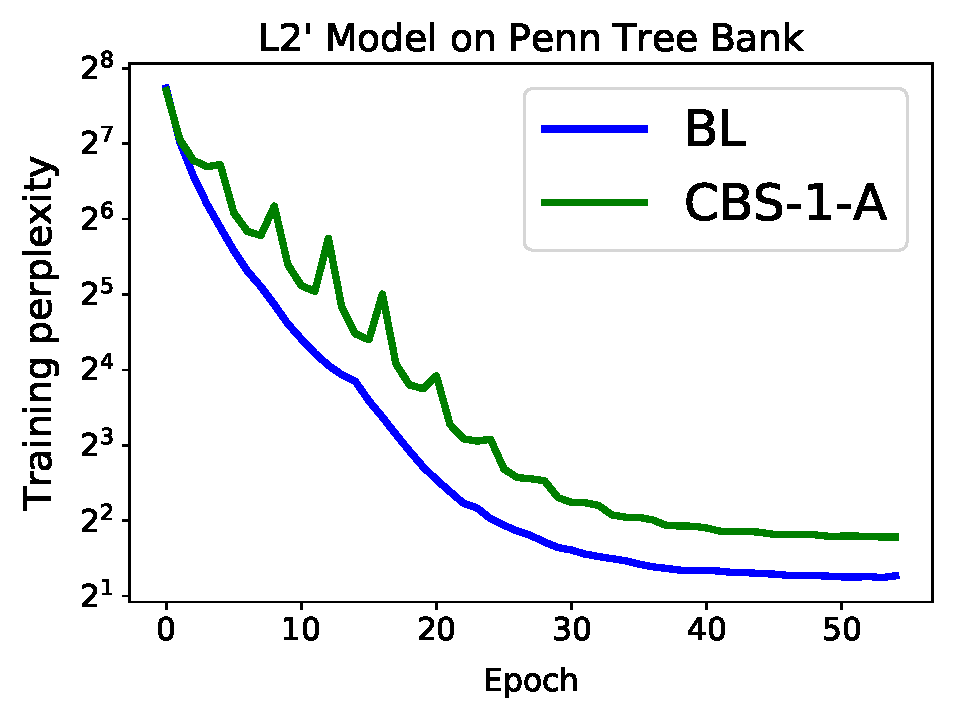
\includegraphics[width=.45\textwidth]{fig/train_l2prime_ptb.pdf}
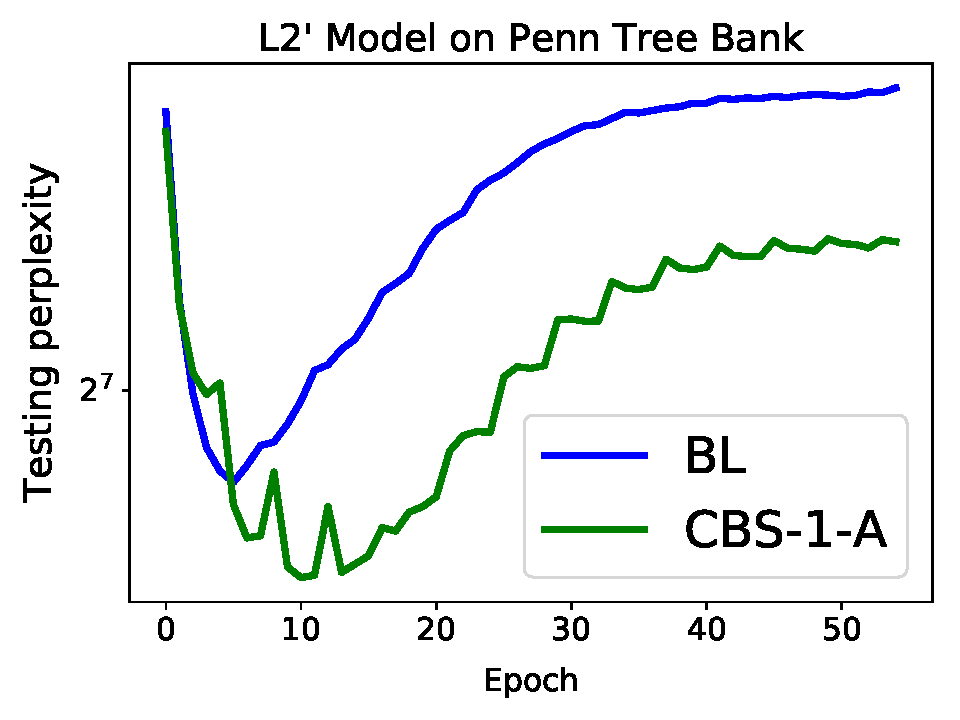
\includegraphics[width=.45\textwidth]{fig/test_l2prime_ptb.pdf}
  \caption{Training (left) and testing (right) perplexity as a function of epoch for overfitting L2' model on Penn Tree Bank.}
  \label{fig:l2'_ptb}
\end{figure}

\begin{figure}[!htbp]
  \centering
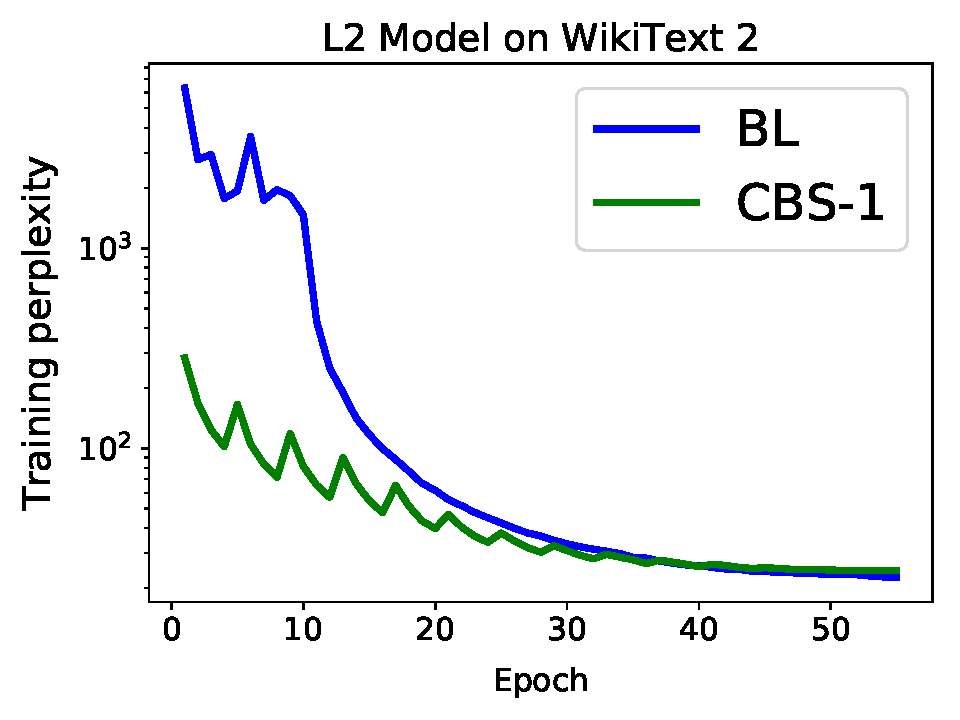
\includegraphics[width=.45\textwidth]{fig/train_l2_wt2.pdf}
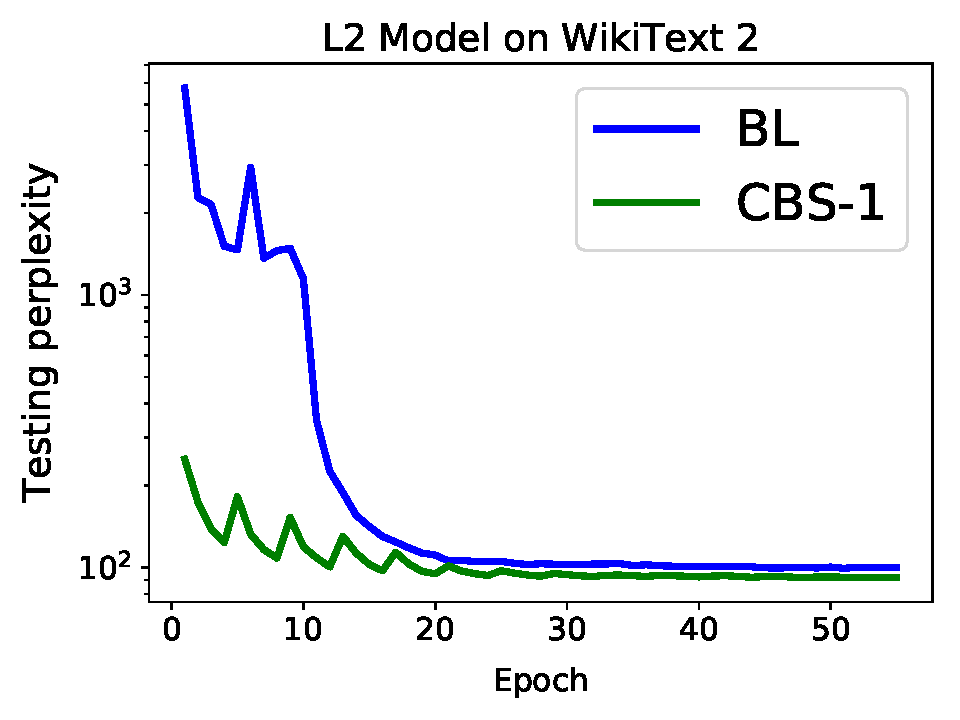
\includegraphics[width=.45\textwidth]{fig/test_l2_wt2.pdf}
  \caption{Training (left) and testing (right) perplexity as a function of epoch for L2 model on WikiText~2.}
  \label{fig:l2_wiki}
\end{figure}
